\documentclass{article}
\usepackage[utf8]{inputenc}
\usepackage[T1]{fontenc}
\usepackage{textcomp}
\usepackage[italian]{babel}
\usepackage{graphicx}
\usepackage{siunitx}
\usepackage{hyperref}
\usepackage{float}
\usepackage{amsmath, amssymb}

\title{Relazione di Laboratorio 1 - Indice di rifrazione del Plexiglas}
\author{Walout Francesco e Iallorenzi Michele}

\begin{document}

\maketitle

\section{Introduzione}
    L'esperimento fatto nel laboratorio dell'ateneo, consiste nel misurare l'indice di rifrazione del plexiglass, attraverso un fit lineare delle misure prese in laboratorio. Cercheremo di spiegare i concetti chiave dell'esperienza e di trarre alcune interessanti conclusioni fisiche riguardo al comportamento della luce.



\section{Esperienza}
    Per il nostro setup-sperimentale, avremo bisogno di una fonte di luce che sia ben collimata, ovvero che la luce non ha delle dispersioni e si presenta come un finissimo raggio (bisogna collimarla in modo tale che la sua luce risulti sottile e distinguibile sulla carta millimetrata). Se si ha a disposizione un laser, la misurazione sarebbe ancora più precisa.
    Prendiamo ora la carta millimetrata e disegniamo due assi cartesiani per fare le nostre misurazioni, infine posizioniamo il cilindro di plexiglas in modo tale che il centro del cilindro coincida con l'origine degli assi.
    Per le misurazioni, sarà necessario puntare la luce verso l'origine del sistema di assi cartesiani, partendo da un generico quadrante con una data angolazione. Ora prendiamo 6 angolazioni diverse della nostra sorgente e tracciamo l'angolo di incidenza e di rifrazione, per ciascuna di esse.

\section{Richiami teorici}
    Spendiamo giusto qualche riga nel parlare della legge che riguarda questo esperimento.

    \subsection{Legge di Snell-Cartesio}
        La legge di Snell-Cartesio, descrive come varia l'angolo di incidenza e l'angolo di rifrazione quando incontra un mezzo che è diverso da quello dove proviene il raggio in origine.
        Il raggio colpisce l'origine del sistema di riferimento che è composto dall'incontro dei due assi "Normale alla superficie" e la superficie stessa. Si generano così due raggi: uno è il Raggio Riflesso ed uno è il Raggio Rifratto. È un dato sperimentale, che vale la seguente relazione:
        \begin{equation}
            n_1 sin(\theta_1) = n_2 sin(\theta_2)
        \end{equation}
        dove: $n_1$ è il mezzo dove passa il raggio incidente, mentre $n_2$ è il mezzo dove passa il raggio rifratto, lo stesso dicasi per gli angoli $\theta_1$ e $\theta_2$.



\section{Elaborazione dei dati}
    Scriviamo un codice Python che prenda in input i dati (angoli di incidenza e di rifrazione) e ci permetta di ottenere una stima dell'indice di rifrazione del Plexiglas ($n_{plx}$).
    Sapendo che l'indice di rifrazione dell'aria è $n_{aria} \sim 1$ possiamo studiare questa funzione:
    \begin{equation}\label{sn}
        n_a sin(\theta_i) = n_{plx} sin(\theta_r) \Rightarrow n_{plx} = \frac{sin(\theta_i)}{sin(\theta_r)}
    \end{equation}
    Siccome le incertezze sugli angoli di incidenza e di rifrazione sono comparabili, non è possibile eseguire in fit dei minimi quadrati (che richiede che la variabile indipendente abbia incertezza trascurabile), per questo calcoliamo direttamente i valori di $n_{plx}$ con l'equazione \ref{sn} e ne facciamo la media pesata con l'inverso delle incertezze quadrate. Questo equivale ad un Fit di una costante, date varie misure di essa.
    I dati sperimentali ed il fit ottenuto, sono mostrati nel grafico \ref{grafico}, il valore ottenuto per $n$ è:
    \begin{gather*}
        n_{media} = 1.45 \pm 0.03
    \end{gather*}
    \begin{figure}[ht!]
        \centering
        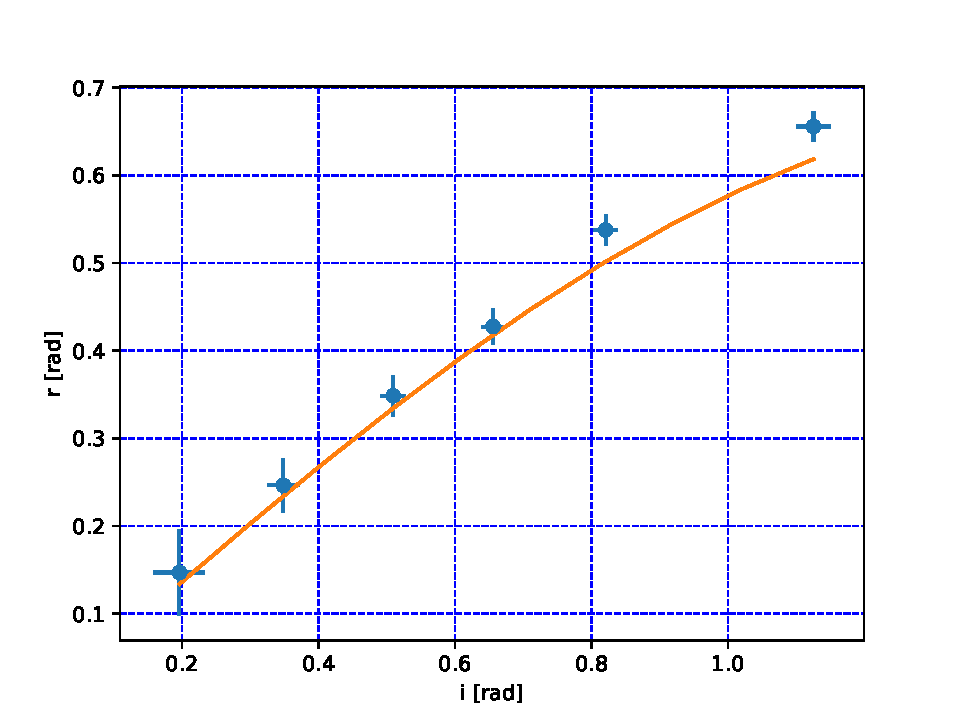
\includegraphics[width=0.8\textwidth]{extra/grafico.pdf}
        \caption{extra/grafico.pdf}
        \label{grafico}
    \end{figure}



\section{Conclusioni}
    Il valore sperimentale dell'indice di rifrazione da noi ottenuto risulta vicino
    a quello che troviamo troviamo online per il plexiglass e il grafico mostra un
    buon accordo rispetto alle misure che abbiamo ottenuto.


\end{document}
